% Created 2016-08-17 Wed 14:38
\documentclass[tikz]{standalone}

\usepackage[utf8]{inputenc}
\usepackage[T1]{fontenc}
\usepackage{helvet}
\usepackage{../../templates/msc}

\renewcommand{\familydefault}{\sfdefault}

\tikzset{
every picture/.style={
line width=1pt
}}

\usepackage{tikz}
\author{Holger Karl}
\date{\today}
\title{}


\begin{document}
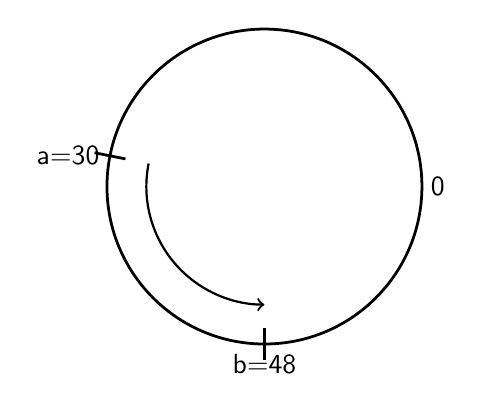
\begin{tikzpicture}[auto, 
block/.style = {rectangle, draw=black, thick, align=left}]

\draw (0,0) circle (2cm);
\node at ({0}:2.2cm) {0}; 
% \node at ({30/64*360}:2.3cm) {a=30}; 
% \node at ({48/64*360}:2.3cm) {b=48}; 
\draw ({30/64*360}:1.8cm)  -- node [left] {a=30} ({30/64*360}:2.2cm); 
\draw ({48/64*360}:1.8cm)  -- node [below] {b=48} ({48/64*360}:2.2cm); 
\draw  [->, thick]({30/64*360}:1.5cm) arc [start angle= {30/64*360}, end angle={48/64*360}, radius=1.5cm];
\end{tikzpicture}
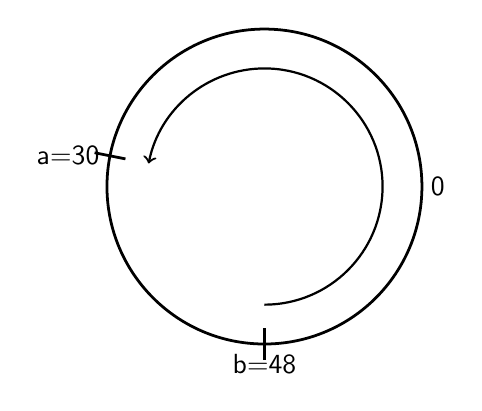
\begin{tikzpicture}[auto, 
block/.style = {rectangle, draw=black, thick, align=left}]

\draw (0,0) circle (2cm);
\node at ({0}:2.2cm) {0}; 
% \node at ({30/64*360}:2.3cm) {a=30}; 
% \node at ({48/64*360}:2.3cm) {b=48}; 
\draw ({30/64*360}:1.8cm)  -- node [left] {a=30} ({30/64*360}:2.2cm); 
\draw ({48/64*360}:1.8cm)  -- node [below] {b=48} ({48/64*360}:2.2cm); 
\draw  [->, thick]({48/64*360}:1.5cm) arc [start angle= {48/64*360}, end angle={30/64*360+360}, radius=1.5cm];
\end{tikzpicture}


% \begin{tikzpicture}
% \draw (0,0) circle (2cm);
%   \draw[red] (330:1.5cm) arc (330:60+360:1.5cm); 
%   \draw[blue] (60:1.2cm) arc (60:330:1.2cm); 
% \end{tikzpicture}

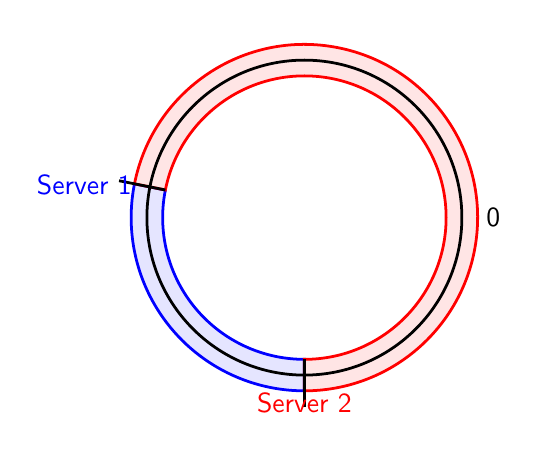
\begin{tikzpicture}[auto, 
block/.style = {rectangle, draw=black, thick, align=left}]


\draw [blue, fill=blue!10] ({30/64*360}:1.8cm) arc ({30/64*360}:{48/64*360}:1.8cm)
--++ ({48/64*360}:0.4cm)  arc ({48/64*360}:{30/64*360}:2.2cm) -- cycle;
\draw [red, fill=red!10] ({48/64*360}:1.8cm) 
arc ({48/64*360}:{30/64*360+360}:1.8cm)
--++ ({30/64*360}:0.4cm)  
arc ({30/64*360+360}:{48/64*360}:2.2cm) -- cycle;


\draw (0,0) circle (2cm);
\node at ({0}:2.4cm) {0}; 
% \node at ({30/64*360}:2.3cm) {a=30}; 
% \node at ({48/64*360}:2.3cm) {b=48}; 

\draw ({30/64*360}:1.8cm)  -- node [left, blue] {Server 1} ({30/64*360}:2.4cm); 
\draw ({48/64*360}:1.8cm)  -- node [below, red] {Server 2} ({48/64*360}:2.4cm); 

\end{tikzpicture}


\end{document}